\section{S-wave observables}
\label{sec:swave:theo:obs}


The angular observables for the P-wave are defined in Section~\ref{sec:kstmm:obs}. 
The inclusion of the S-wave in the complete angular distribution means 
that \AFB can no longer be determined by 
experimentally counting the number of events with forward-going and  
backward-going leptons, as Eqs.~\ref{eq:theoafb} and~\ref{eq:expafb} 
are no longer equivalent. 
This is because the total normalisation for the angular distribution changes to the 
sum of S- and P-wave amplitudes,
\begin{align}
\Gamma^{''}  &\equiv \frac{\deriv^2\Gamma}{\deriv\psq\deriv\qsq} =   |A_{10}|^2 + |A_{1||}|^2 + |A_{1\bot}|^2 + |A_{00}|^2 .
\end{align}
such that there is a factor of 
\begin{align} 
\FPi(\psq,\qsq) &= \left( \frac{|A_{10}|^2 + |A_{1||}|^2 + |A_{1\bot}|^2 }
{|A_{10}|^2 + |A_{1||}|^2 + |A_{1\bot}|^2 + |A_{00}|^2} \right)
\end{align}
between the pure P-wave and the admixture of the S- and the P-wave. This is the fraction of the yield coming 
from the P-wave at a given value of \psq and \qsq. 
Similarly, the S-wave fraction is defined as 
\begin{align}
\FSi(\psq,\qsq) &= \left( \frac{|A_{00}|^2}{|A_{10}|^2 + |A_{1||}|^2 + |A_{1\bot}|^2 + |A_{00}|^2} \right)
\end{align}
and the interference between the S-wave and the P-wave as 
\begin{align}
\ASi(\psq,\qsq)  &= \frac{\sqrt{3}}{2} \left( \frac{ |A_{0L0}||A_{1L0}|\cos\delta_L
+ (L\to R)}{|A_{10}|^2 + |A_{1||}|^2 + |A_{1\bot}|^2 + |A_{00}|^2}\right) \, .
\end{align}
Substituting the above observables into the angular terms gives 
\begin{align}
\label{eq:angularcoeffwithobs}
\frac{I_1^c}{\Gamma^{''}} &=  \frac{1}{4\pi} \FSi + \frac{3}{4\pi} \FPi \FL \ctksq +  \frac{3}{4\pi} \ASi \ctk  \nonumber \\
\frac{I_1^s}{\Gamma^{''}} &= \frac{3}{4} \frac{3}{8\pi} \FPi \left( 1 - \FL \right)  \left(1-\ctksq\right)   \nonumber \\
\frac{I_2^c}{\Gamma^{''}} &= -  \left( \frac{1}{4\pi} \right. \FSi + \frac{3}{4\pi} \FPi\left( 1 - \FL \right) \ctksq +\left.   \frac{3}{4\pi} \ASi \ctk \ctk \right)  ,\nonumber \\
\frac{I_2^s}{\Gamma^{''}} &= \frac{1}{4}   \frac{3}{8\pi}  \FPi\left( 1 - \FL \right)  \left(1-\ctksq\right)    \\
\frac{I_3}{\Gamma^{''}} &= \frac{1}{2}  \frac{3}{8\pi}  \FPi  \AT2   \left(1-\ctksq\right)   \nonumber \\
\frac{I_6}{\Gamma^{''}} &= 2  \frac{3}{8\pi} \frac{4}{3} \FPi  \AFB   \left(1-\ctksq\right)   \nonumber \\
\frac{I_9}{\Gamma^{''}} &=    \frac{3}{8\pi}  \FPi \AIm \left(1-\ctksq\right)    \, .\nonumber 
\end{align}
 Following what is described in Section~\ref{sec:fullangdist}, 
simplification of the angular distribution can be achieved by folding
 the distribution in $\phi$ such that $\phiprime = \phi - \pi $ 
for $\phi < 0 $~\cite{Ksteepubnote}.
The $I_{4,5,7,8}$ angular terms which are dependent on $\cos\phi$ or
$\sin\phi$ are cancelled, leaving $I_{1,2,3,6}$, in the angular distribution:
\begin{align}
\label{eq:folded}
\frac{\text{d}^5\Gamma}{\text{d}q^2 \text{d}p^2 \dctk \dctl
\text{d}\phiprime} = & \frac{3}{8} \left( I_1^c + 2I_1^s + (I_2^c + 2I_2^s)
\cos2\theta_l  + 2I_3\stlsq\cos2\phiprime \right. \nonumber \\
& \left. + 2I_6\ctl + 2\sqrt{2}I_9\stlsq\sin2\phiprime \frac{}{} \right) .
\end{align}

Combining Equation~\ref{eq:folded} with~\ref{eq:angularcoeffwithobs} gives the differential decay distribution,
\begin{equation}
\label{eq:theo5d}
\begin{split}
\frac{1}{\Gamma^{''}} \frac{\text{d}^5\Gamma}{\text{d}\qsq\text{d}\psq \dctk
\dctl \text{d}\phiprime} =   \frac{9}{16\pi}   \Bigg( & \left(  \frac{2}{3}\FSi  +  \frac{4}{3} \ASi \ctk \right) ( 1 - \ctlsq )    \\
& \quad + \FPi  \bigg[\xspace 2 \FL \ctksq ( 1 - \ctlsq )   \\ 
& \quad \quad + \frac{1}{2} ( 1 - \FL ) ( 1 - \ctksq ) ( 1 + \ctlsq )  \\
& \quad \quad + \frac{1}{2} ( 1 - \FL ) \AT2 ( 1 - \ctksq ) (  1 - \ctlsq )
\cos2\phiprime  \\
& \quad \quad +  \frac{4}{3} \AFB ( 1 - \ctksq ) \ctl  \\ 
& \quad \quad + \AIm ( 1 - \ctksq ) ( 1 - \ctlsq) \sin2\phiprime  \bigg]  \Bigg) . 
\end{split}
\end{equation}
which is a combination of the P-wave observables and the transverse angular observables.
%This is the angular distribution used in Chapter 5.
The angular distribution as a function of \ctl  and \ctk is given by integrating over $\phi$ in Eq.~\ref{eq:theo5d}
\begin{equation}
\label{eq:theo4d}
\begin{split}
\frac{1}{\Gamma^{''}} \frac{\text{d}^4\Gamma}{\text{d}\qsq\text{d}\psq\text{d}
\ctk \text{d}\ctl} =   \frac{9}{16} & \Bigg( \left( \frac{2}{3} \FSi + \frac{4}{3} \ASi \ctk \right) ( 1 - \ctlsq )  \\
&+ \FPi  \bigg[  2 \FL \ctksq ( 1 - \ctlsq )  \\ 
& \quad \ +\frac{1}{2}  ( 1 - \FL ) ( 1 - \ctksq ) ( 1 + \ctlsq )  \\
& \quad \ + \frac{4}{3} \AFB ( 1 - \ctksq ) \ctl   \bigg]  \Bigg) 
\end{split}
\end{equation}
and further integration from Equation~\ref{eq:theo5d} yields the angular distribution for each of the angles,
\begin{equation}
\label{eq:theo3d}
\begin{split}
\frac{1}{\Gamma^{''}} \frac{\text{d}^3\Gamma}{\text{d}\qsq\text{d}\psq\dctl}
&=  \frac{3}{4} \FSi ( 1 - \ctlsq ) + \FPi  \bigg[  \frac{3}{4} \FL ( 1 - \ctlsq ) \\
&  + \frac{3}{8} ( 1 - \FL ) ( 1 + \ctlsq ) + \AFB \ctl  \bigg]  , \\
\frac{1}{\Gamma^{''}} \frac{\text{d}^3\Gamma}{\text{d}\qsq\text{d}\psq\dctk 
} &=   \frac{1}{2} \FSi + \ASi \ctk \\&
+ \FPi \bigg[ \frac{3}{2}  \FL \ctksq +  \frac{3}{4} ( 1 - \FL ) ( 1 - \ctksq ) \bigg] 	, \\
\frac{1}{\Gamma^{''}} \frac{\text{d}^3\Gamma}{\text{d}\qsq\text{d}\psq\text{d}\phiprime
} &= \frac{1}{\pi} \Bigg(  1 + \frac{3}{4} \FSi    + \FPi \bigg[\xspace   \FL  
+ \frac{1}{2} ( 1 - \FL ) \AT2  \cos2\phiprime +  \OS{3}  \sin2\phiprime  \bigg]  \Bigg) .
\end{split}
\end{equation}
\subsubsection{Angular distribution integrated over \psq}
The angular distribution can be integrated over \psq using the weighted integral 
\begin{align}
\label{eq:obsint}
O(\qsq) &=  \frac{ \int \mathcal{O}(\psq,\qsq) \frac{\text{d}^2\Gamma}
{\text{d}\psq\text{d}\qsq} \text{d}\psq }{ \int  \frac{\text{d}^2\Gamma}
{\text{d}\psq\text{d}\qsq} \text{d}\psq }
\end{align}
for the value of the observables integrated over a given region in \psq. 
This leads to the integrated observables \FP, \FS and \AS which are solely 
dependant on \qsq. By definition, the fraction of the S-wave and the P-wave
 sum to one, $\FS + \FP = 1$.
The complete angular distribution without any \psq dependence is given by
\begin{align}
\label{eq:theo4dint}
\frac{1}{\Gamma^{'}} \frac{\text{d}^5\Gamma}{\text{d}\qsq\dctk
\dctl \text{d}\phiprime} =   \frac{9}{16\pi}  & \Bigg( \left( \frac{2}{3} \FS +  \frac{4}{3} \AS \ctk \right) ( 1 - \ctlsq )   \nonumber \\
&+ (1-\FS)  \bigg[\xspace 2 \FL \ctksq ( 1 - \ctlsq )  \nonumber \\ 
&  \quad \quad \quad  + \frac{1}{2} ( 1 - \FL ) ( 1 - \ctksq ) ( 1 + \ctlsq )  \nonumber \\
&  \quad \quad \quad  + \frac{1}{2} ( 1 - \FL ) \AT2 ( 1 - \ctksq ) (  1 - \ctlsq ) \cos2\phiprime  \nonumber \\
&  \quad \quad \quad  +  \frac{4}{3} \AFB ( 1 - \ctksq ) \ctl  \nonumber \\ 
&  \quad \quad \quad  + \OS{3} ( 1 - \ctksq ) ( 1 - \ctlsq) \sin2\phiprime  \bigg] \Bigg) . 
\end{align}
 where the normalisation of the angular distribution is given by 
\begin{align}
\Gamma^{'} = \frac{\deriv\Gamma}{\deriv\qsq} \, .
\end{align}
The `dilution' effect of the S-wave can clearly be seen from the factor of $(1-\FS)$ that appears in front of the  observables in Eq.~\ref{eq:theo4dint}. 


The effect of an S-wave on the angular distribution as a function of \ctk, \ctl and \phiprime is illustrated in Fig.~\ref{fig:1dcalc}. 
\begin{figure}[tp]
\centering
\hspace{-0.2in}
\subfigure[]{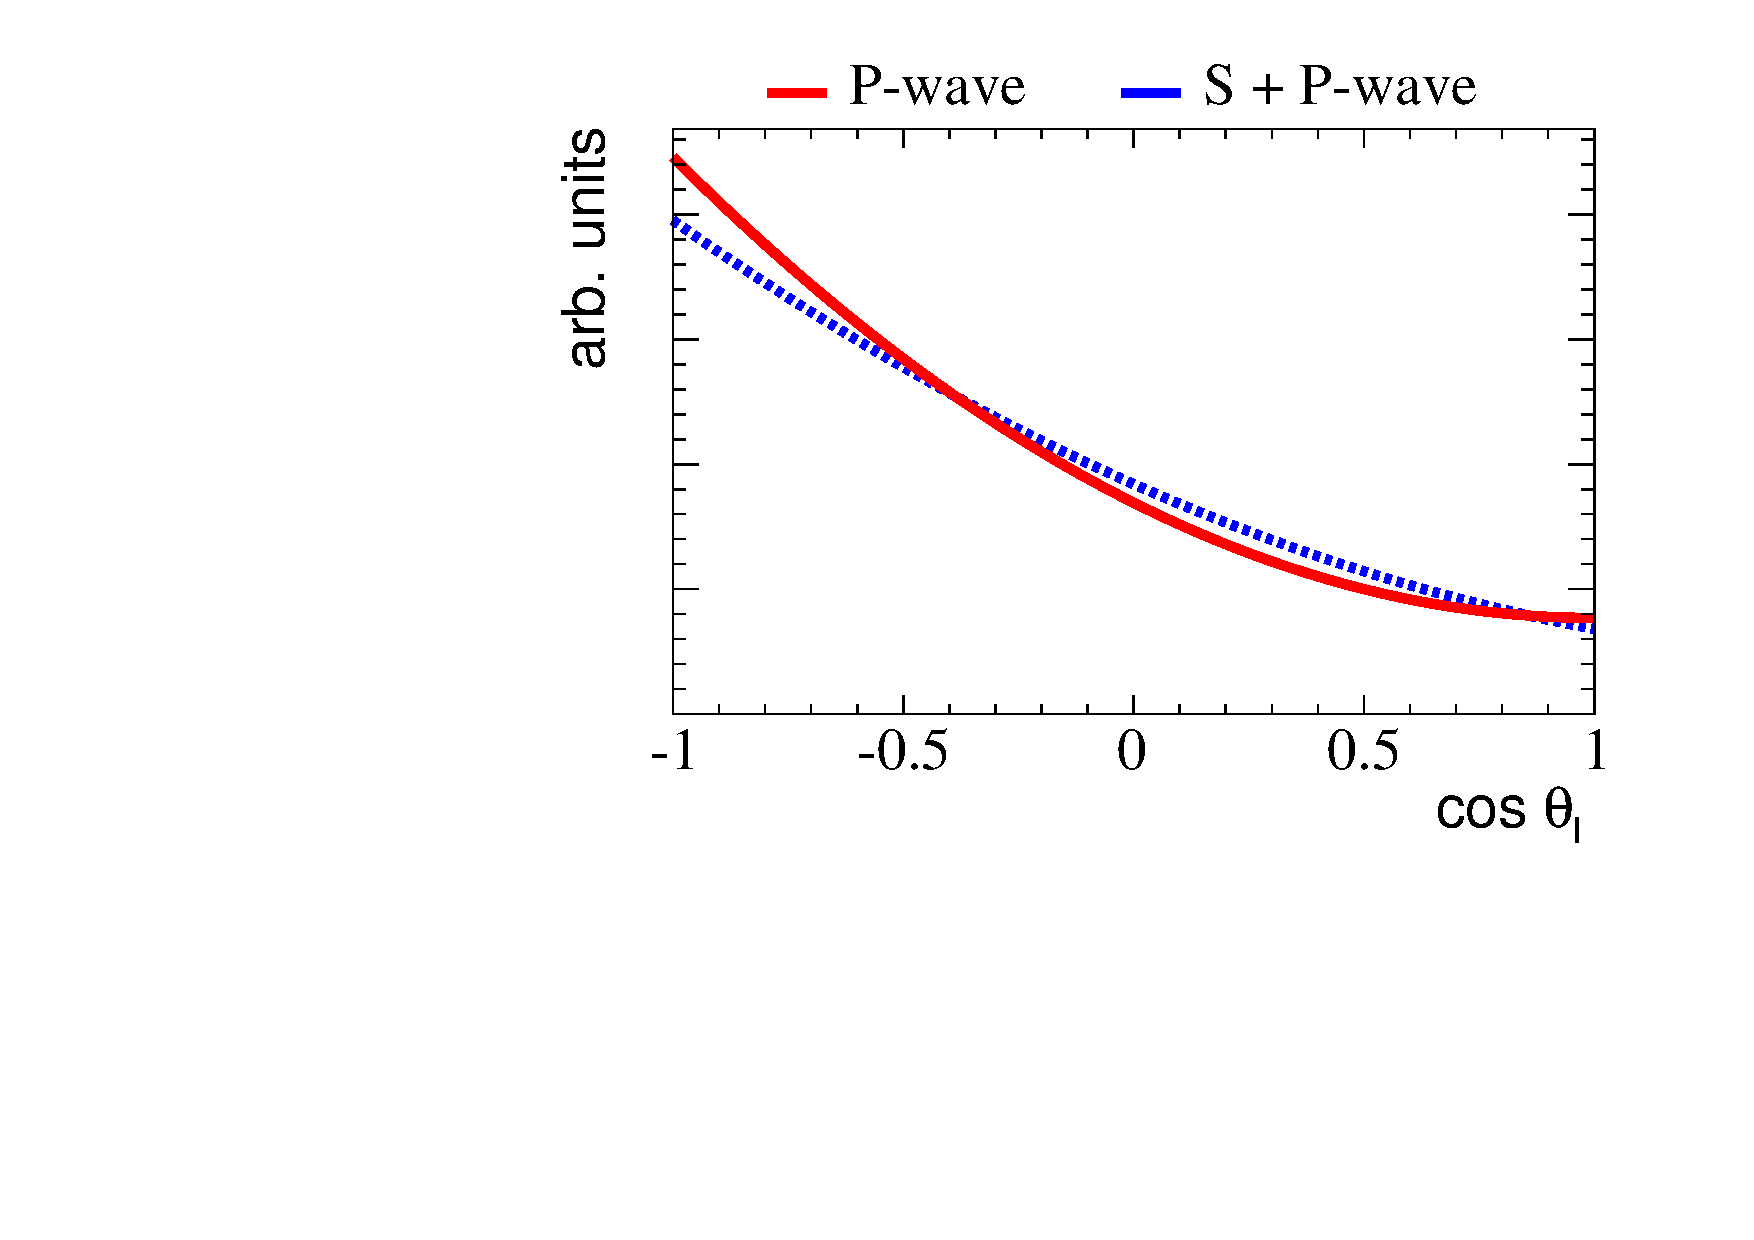
\includegraphics[width=0.48\textwidth]{chapter6/figs/test_pdfs_swave_ctl.pdf}}
\subfigure[]{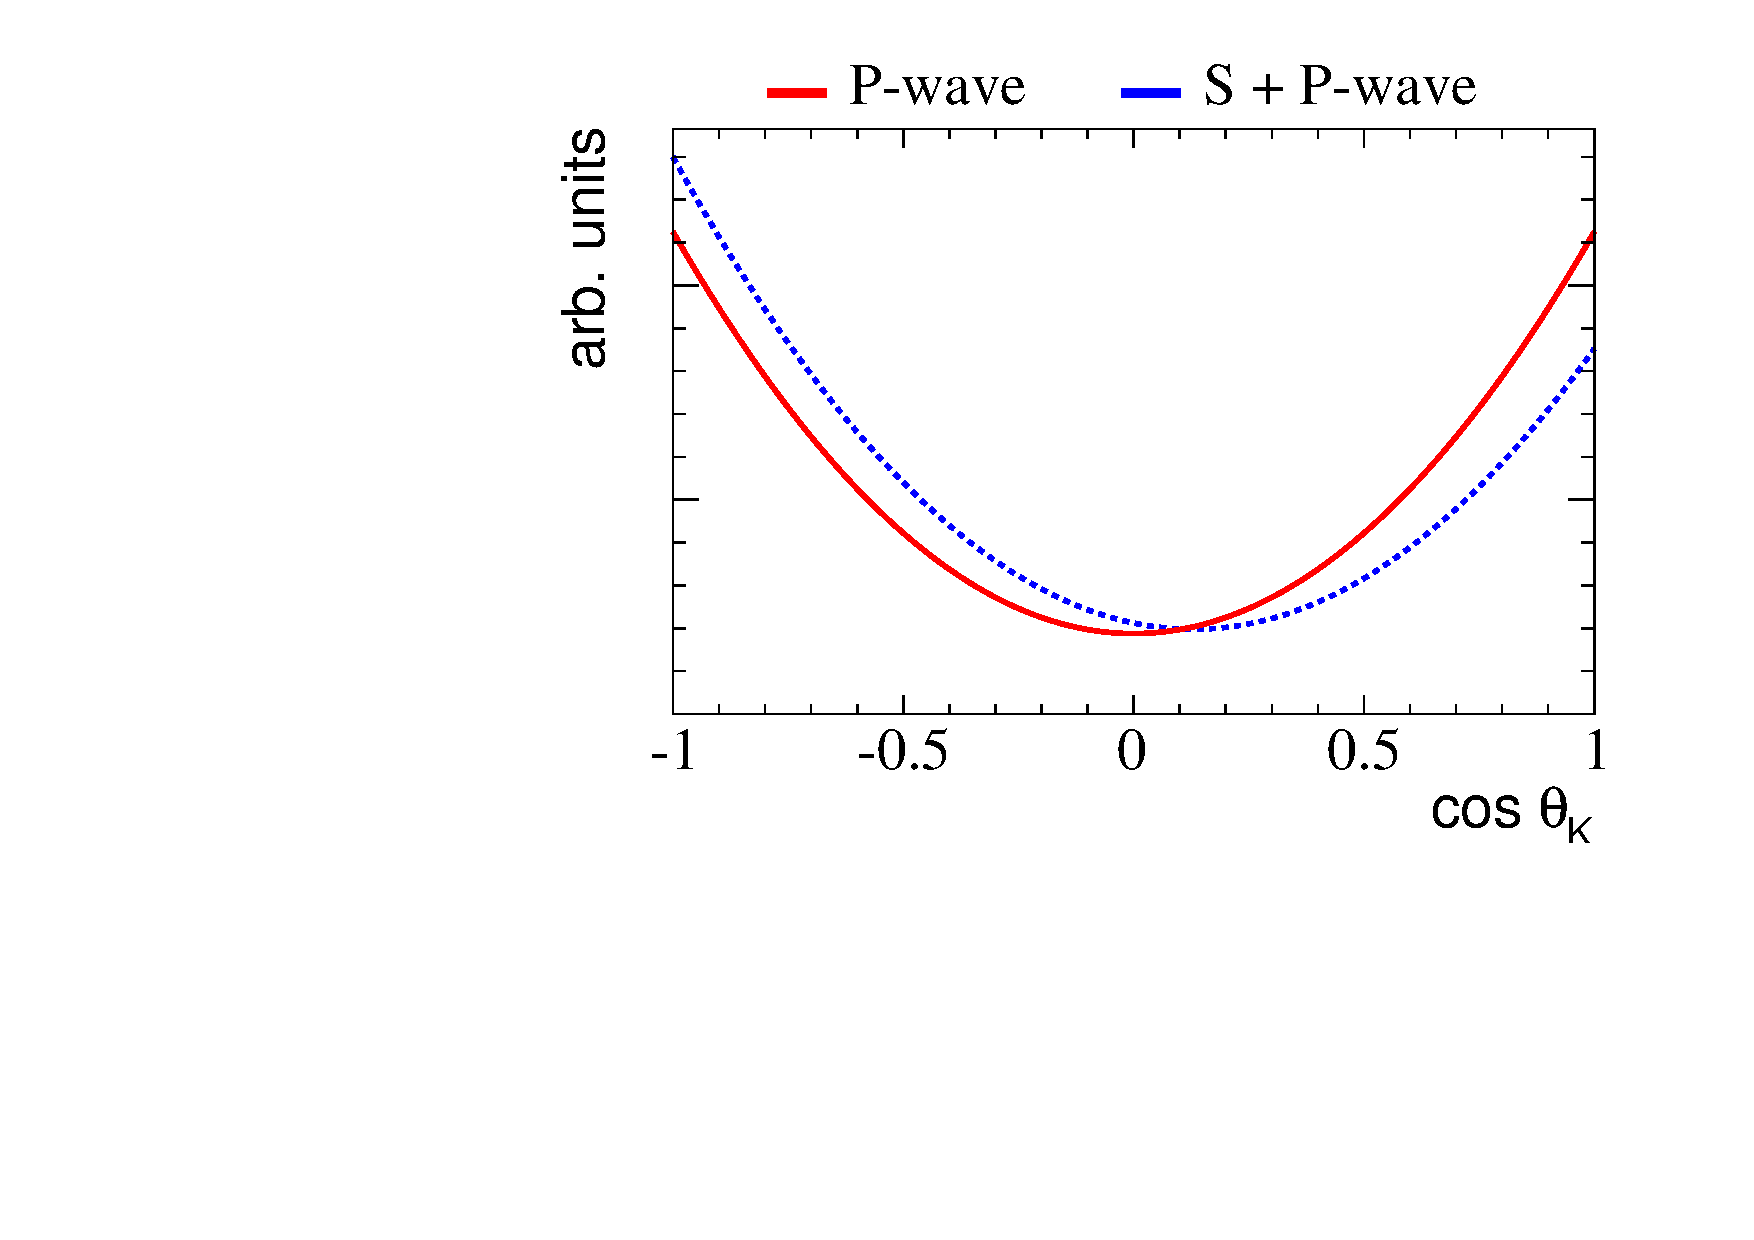
\includegraphics[width=0.48\textwidth]{chapter6/figs/test_pdfs_swave_ctk.pdf}}
\subfigure[]{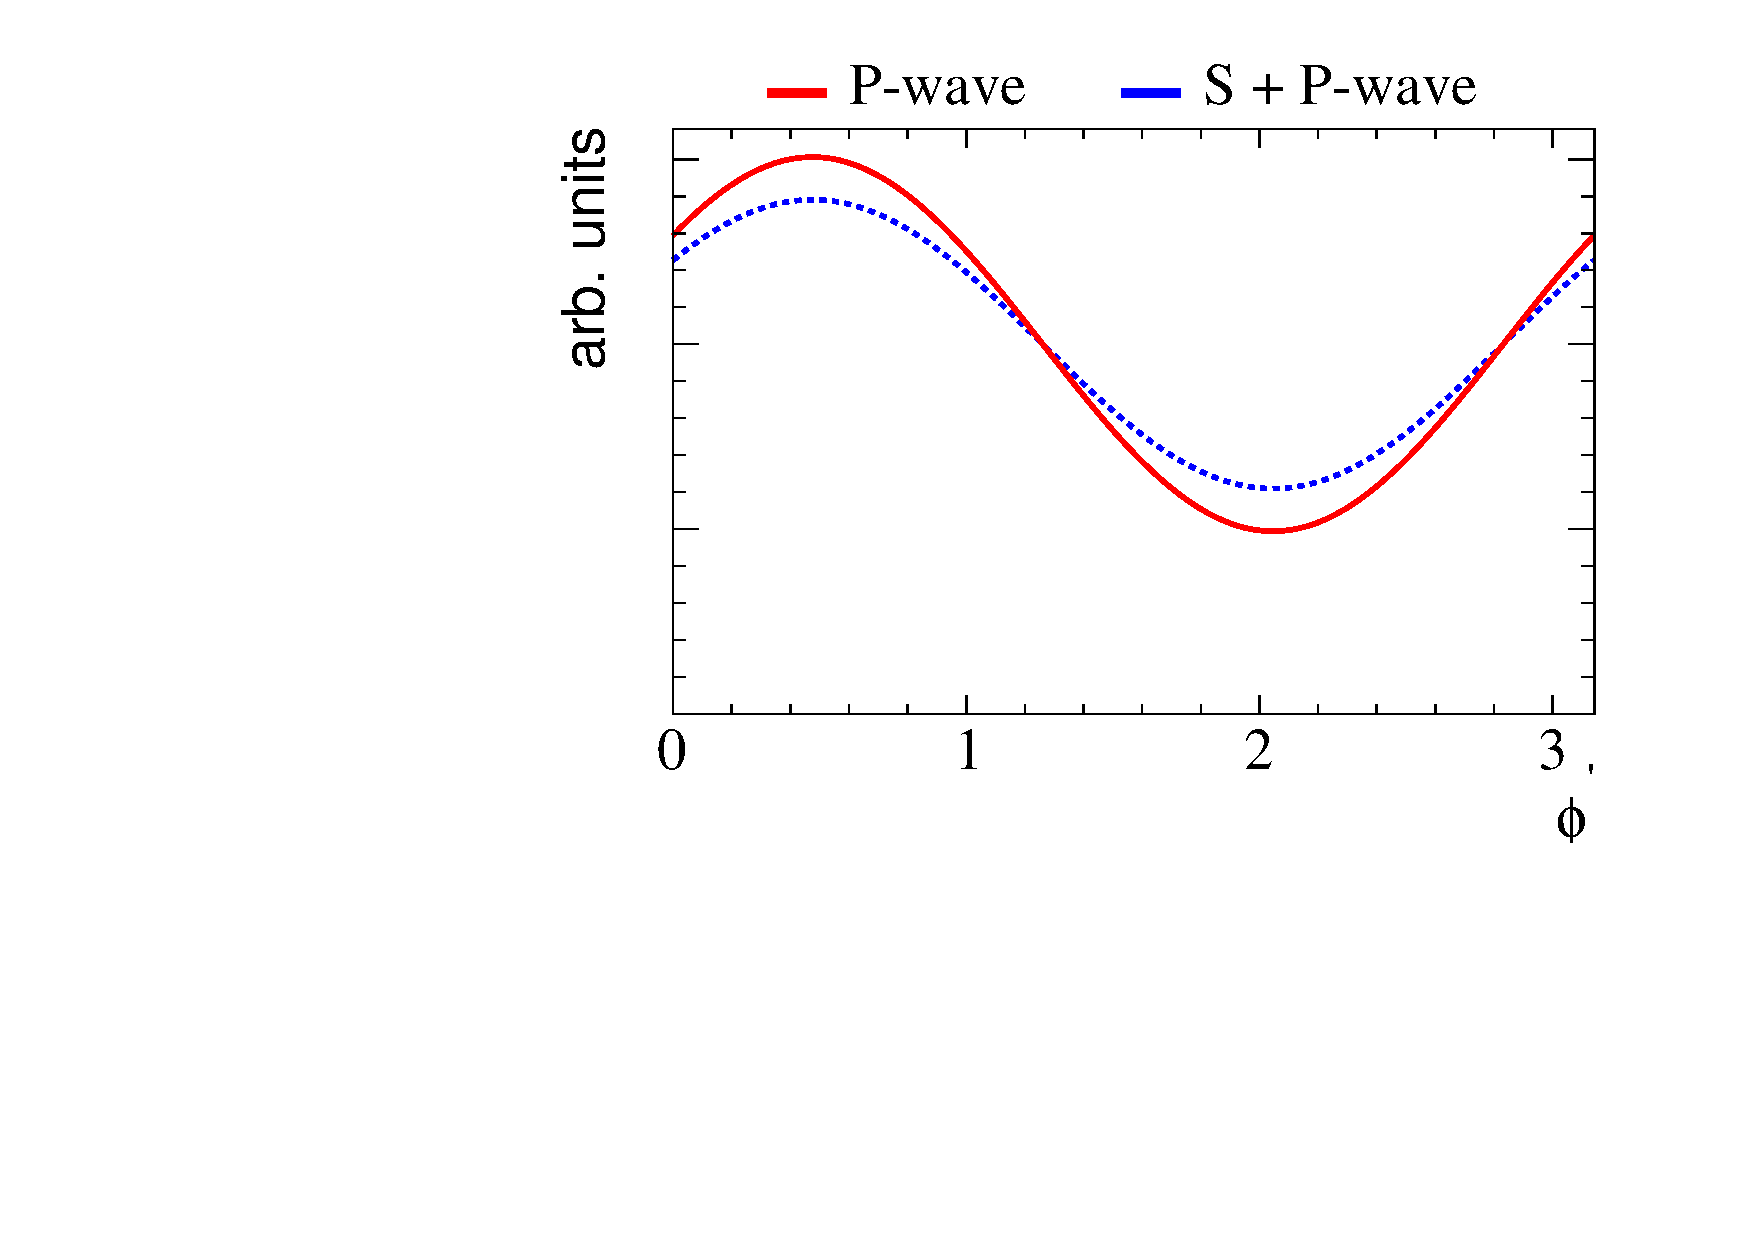
\includegraphics[width=0.48\textwidth]{chapter6/figs/test_pdfs_swave_phi.pdf}}
\caption[  The effect of the S-wave on \ctk, \ctl and \phiprime.    ]
{One-dimensional projections of (a) \ctl, (b) \ctk, (c) \phiprime 
for the angular distribution of \BdToKstll with (blue-dashed) and without (red-solid) an 
S-wave component of 7\%. The dilution effect of the S-wave on the asymmetry 
in \ctl and the asymmetric effect in \ctk can be clearly seen.~\label{fig:1dcalc}}
\end{figure}
Here it is possible to see that the asymmetry in \ctl, given by \AFB, 
has decreased and that there is an asymmetry in \ctk introduced by the interference term.




